% =============================================================================
% Autore originale: Fabio Tempera
% Licenza: MIT (vedere LICENSE nel medesimo direttorio)
%
% DOCUMENTO
%   Proposta ufficiale di collaborazione per la rete TESS-4C in Abruzzo,
%   da inviare a istituti scolastici, enti parco e dipartimenti universitari.
%   Preambolo comune (fenomeno, osservabile, strumento, installazione) e
%   seconda parte distinta per interlocutore. L'elenco dei siti candidati
%   resta nel resoconto interno, non in questa lettera.
%
% COMPILAZIONE
%   pdflatex proposta-template.tex  (due passate per i riferimenti a Figure e Tabelle)
%   Classe report, pacchetti in packages.sty. Non usare Markdown.
% =============================================================================

\documentclass[11pt,a4paper]{report}

\usepackage{packages}

\definecolor{nightblue}{RGB}{22,38,58}
\definecolor{steel}{RGB}{80,100,120}
\definecolor{linegray}{RGB}{200,200,200}

\renewcommand{\thesection}{\arabic{section}}
\renewcommand{\thefigure}{\arabic{figure}}
\renewcommand{\thetable}{\arabic{table}}
\setcounter{secnumdepth}{0}

\titleformat{\section}
  {\normalfont\Large\bfseries\color{nightblue}}
  {\thesection}{0.6em}{}
\titleformat{\subsection}
  {\normalfont\large\bfseries\color{nightblue}}
  {\thesubsection}{0.6em}{}
\titlespacing{\section}{0pt}{1.4em}{0.6em}
\titlespacing{\subsection}{0pt}{1.1em}{0.4em}

\pagestyle{fancy}
\fancyhf{}
\renewcommand{\headrulewidth}{0.4pt}
\renewcommand{\headrule}{\hbox to\headwidth{\color{linegray}\leaders\hrule height \headrulewidth\hfill}}
\fancyhead[L]{\small\color{steel} CieloBuio OdV}
\fancyhead[R]{\small\color{steel} Proposta di collaborazione TESS-4C Abruzzo}
\fancyfoot[C]{\small\color{steel}\thepage}

\hypersetup{
  colorlinks=true,
  linkcolor=nightblue,
  urlcolor=nightblue,
  citecolor=nightblue,
  pdftitle={Proposta di collaborazione. Rete TESS-4C Abruzzo},
  pdfauthor={Fabio Tempera}
}

\setlist[itemize]{leftmargin=1.4em, itemsep=0.25em, topsep=0.3em}
\setlist[enumerate]{leftmargin=1.6em, itemsep=0.25em, topsep=0.3em}

\newcommand{\infobox}[1]{%

  \begin{center}

  \renewcommand{\arraystretch}{1.5}

  \begin{tabularx}{\linewidth}{X}
    \arrayrulecolor{linegray}
    \toprule
    #1 \\
    \bottomrule
  \end{tabularx}

  \end{center}

}

\begin{document}

\begin{center}

{\LARGE\bfseries\color{nightblue} Una stazione fotometrica per il monitoraggio del cielo notturno\par}

\vspace{0.2cm}

{\large Proposta di collaborazione per scuole, enti parco e atenei dell'Abruzzo\par}

\vspace{0.1cm}

{\small CieloBuio OdV, progetto rete TESS-4C}

\end{center}

% Preambolo comune: vale per scuola, parco e ateneo.
\section*{Oggetto}
\addcontentsline{toc}{section}{Oggetto}

La presente proposta invita l'ente destinatario a ospitare, in autonomia e senza vincoli esterni, una stazione di misura della qualità del cielo notturno. La stazione entra nella rete TESS-4C in via di costituzione in Abruzzo, parte del progetto di CieloBuio OdV.

Il testo introduce il fenomeno, l'osservabile e lo strumento, poi si rivolge in modo distinto a istituto scolastico, ente parco e dipartimento universitario. Resta una lettera unica, da inviare così com'è.

Lo strumento previsto è il fotometro multibanda \textit{TESS-4C}. I dati confluiscono in un repository aperto (rete STARS4ALL) e in un cruscotto della rete abruzzese, con accesso ai dati grezzi per didattica, tutela ambientale e ricerca.

\infobox{%
\textit{In sintesi}: un investimento una tantum di circa 550-650 EUR per lo strumento, alimentazione a 5\,V, connessione WiFi, un'installazione affidata a un tecnico dell'ente ospitante, e una serie storica georeferenziata di brillanza superficiale del cielo.
}

\section*{L'inquinamento luminoso}
\addcontentsline{toc}{section}{L'inquinamento luminoso}

L'inquinamento luminoso è un problema globale che, al pari di altre forme di inquinamento di origine antropica, produce effetti sugli ecosistemi e sugli organismi viventi. Il dibattito è nato nella comunità astronomica professionale, preoccupata che l'uso inefficiente, superfluo e non controllato della luce artificiale notturna (\textit{artificial light at night}, ALAN) potesse compromettere la visibilità del cielo stellato dagli osservatori. Oggi lo stesso fenomeno è oggetto di ricerca interdisciplinare, di studi socioeconomici e di un dibattito culturale sul cielo notturno come patrimonio.

Gli effetti della luce artificiale notturna sono legati allo sviluppo e all'uso improprio di sorgenti sempre più efficienti e spesso più economiche. Negli anni 70 la transizione in discussione era quella dalle lampade al mercurio a quelle al sodio ad alta pressione. Oggi è in corso un passaggio verso i diodi a emissione di luce (LED). La distribuzione spettrale di potenza è cambiata: da poche righe di emissione si è passati a un numero elevato di componenti, con un continuo più intenso soprattutto nel blu e nel verde.

A questa transizione si accompagna un aumento della luce artificiale a quasi tutte le scale spaziali. Si stima che circa il 99\% della popolazione di Stati Uniti ed Europa viva sotto un cielo inquinato, e che più del 33\% della popolazione mondiale non possa più osservare la Via Lattea (Falchi et al., 2016). Nemmeno le aree remote sono immuni: la luce artificiale si propaga nell'atmosfera e produce un alone visibile a grande distanza dalla sorgente.

I dati oggettivi e accessibili sono la base per qualsiasi norma di mitigazione e per misurarne l'efficacia. In Italia diverse regioni dispongono di leggi sul contenimento della luce artificiale. In assenza di reti di misura a terra, il monitoraggio si appoggia spesso a stime satellitari, poco puntuali rispetto a una stazione in sito. Il progetto CieloBuio propone una rete di stazioni su base volontaria, anche in Abruzzo, dove la luce artificiale notturna è oggetto di disciplina regionale.

Il preambolo di questa sezione è stato riadattato da rassegne e articoli di riferimento sulla luce artificiale notturna, in particolare Chepesiuk (2009), Bennie et al.\ (2015), Irwin (2018), Svechkina et al.\ (2020), Walker (1970), Riegel (1973), DiLaura (2008), Kyba et al.\ (2017 e 2023), Sánchez de Miguel et al.\ (2021) e Falchi et al.\ (2016). Per lo strumento TESS il riferimento tecnico è Zamorano et al.\ (2016); per il Day/Night Band di VIIRS, Liao et al.\ (2013). L'elenco bibliografico esteso non viene riportato, per non appesantire un testo destinato a un uso operativo.

\section*{Cosa si misura}
\addcontentsline{toc}{section}{Cosa si misura}

Uno strumento fotometrico \textit{non} misura l'inquinamento luminoso. L'osservabile è una \textit{brillanza superficiale} del cielo, cioè la quantità di luce che arriva da una porzione di volta celeste. La brillanza si esprime in candele per metro quadro oppure, in modo equivalente, in magnitudini per arcosecondo quadro in una banda passante definita.

Quella brillanza è la somma di un contributo naturale, sempre presente anche nei cieli più inquinati, e di un contributo artificiale. Il contributo naturale comprende fattori di origine astronomica (luce stellare integrata, polvere interstellare, luce zodiacale) e fattori atmosferici, in primo luogo l'\textit{airglow}. Il contributo artificiale è la luce emessa a terra, diffusa e riflessa dall'atmosfera. Distinguere le 2 componenti, e interpretare i dati, è il lavoro dell'esperto. L'esperienza associativa di CieloBuio è, in questo passaggio, il valore aggiunto rispetto alla sola lettura dello strumento.

La Figura~\ref{fig:contributi} schematizza il punto, in unità arbitrarie: il fotometro registra la somma. In un sito di alta quota il contributo artificiale è piccolo; in un centro urbano domina.

\begin{figure}[ht!]
\centering
% Figura: scripts/generate_contributi.py (repo tess4c-figure-scripts). Schema didattico nello script, non un JSON.
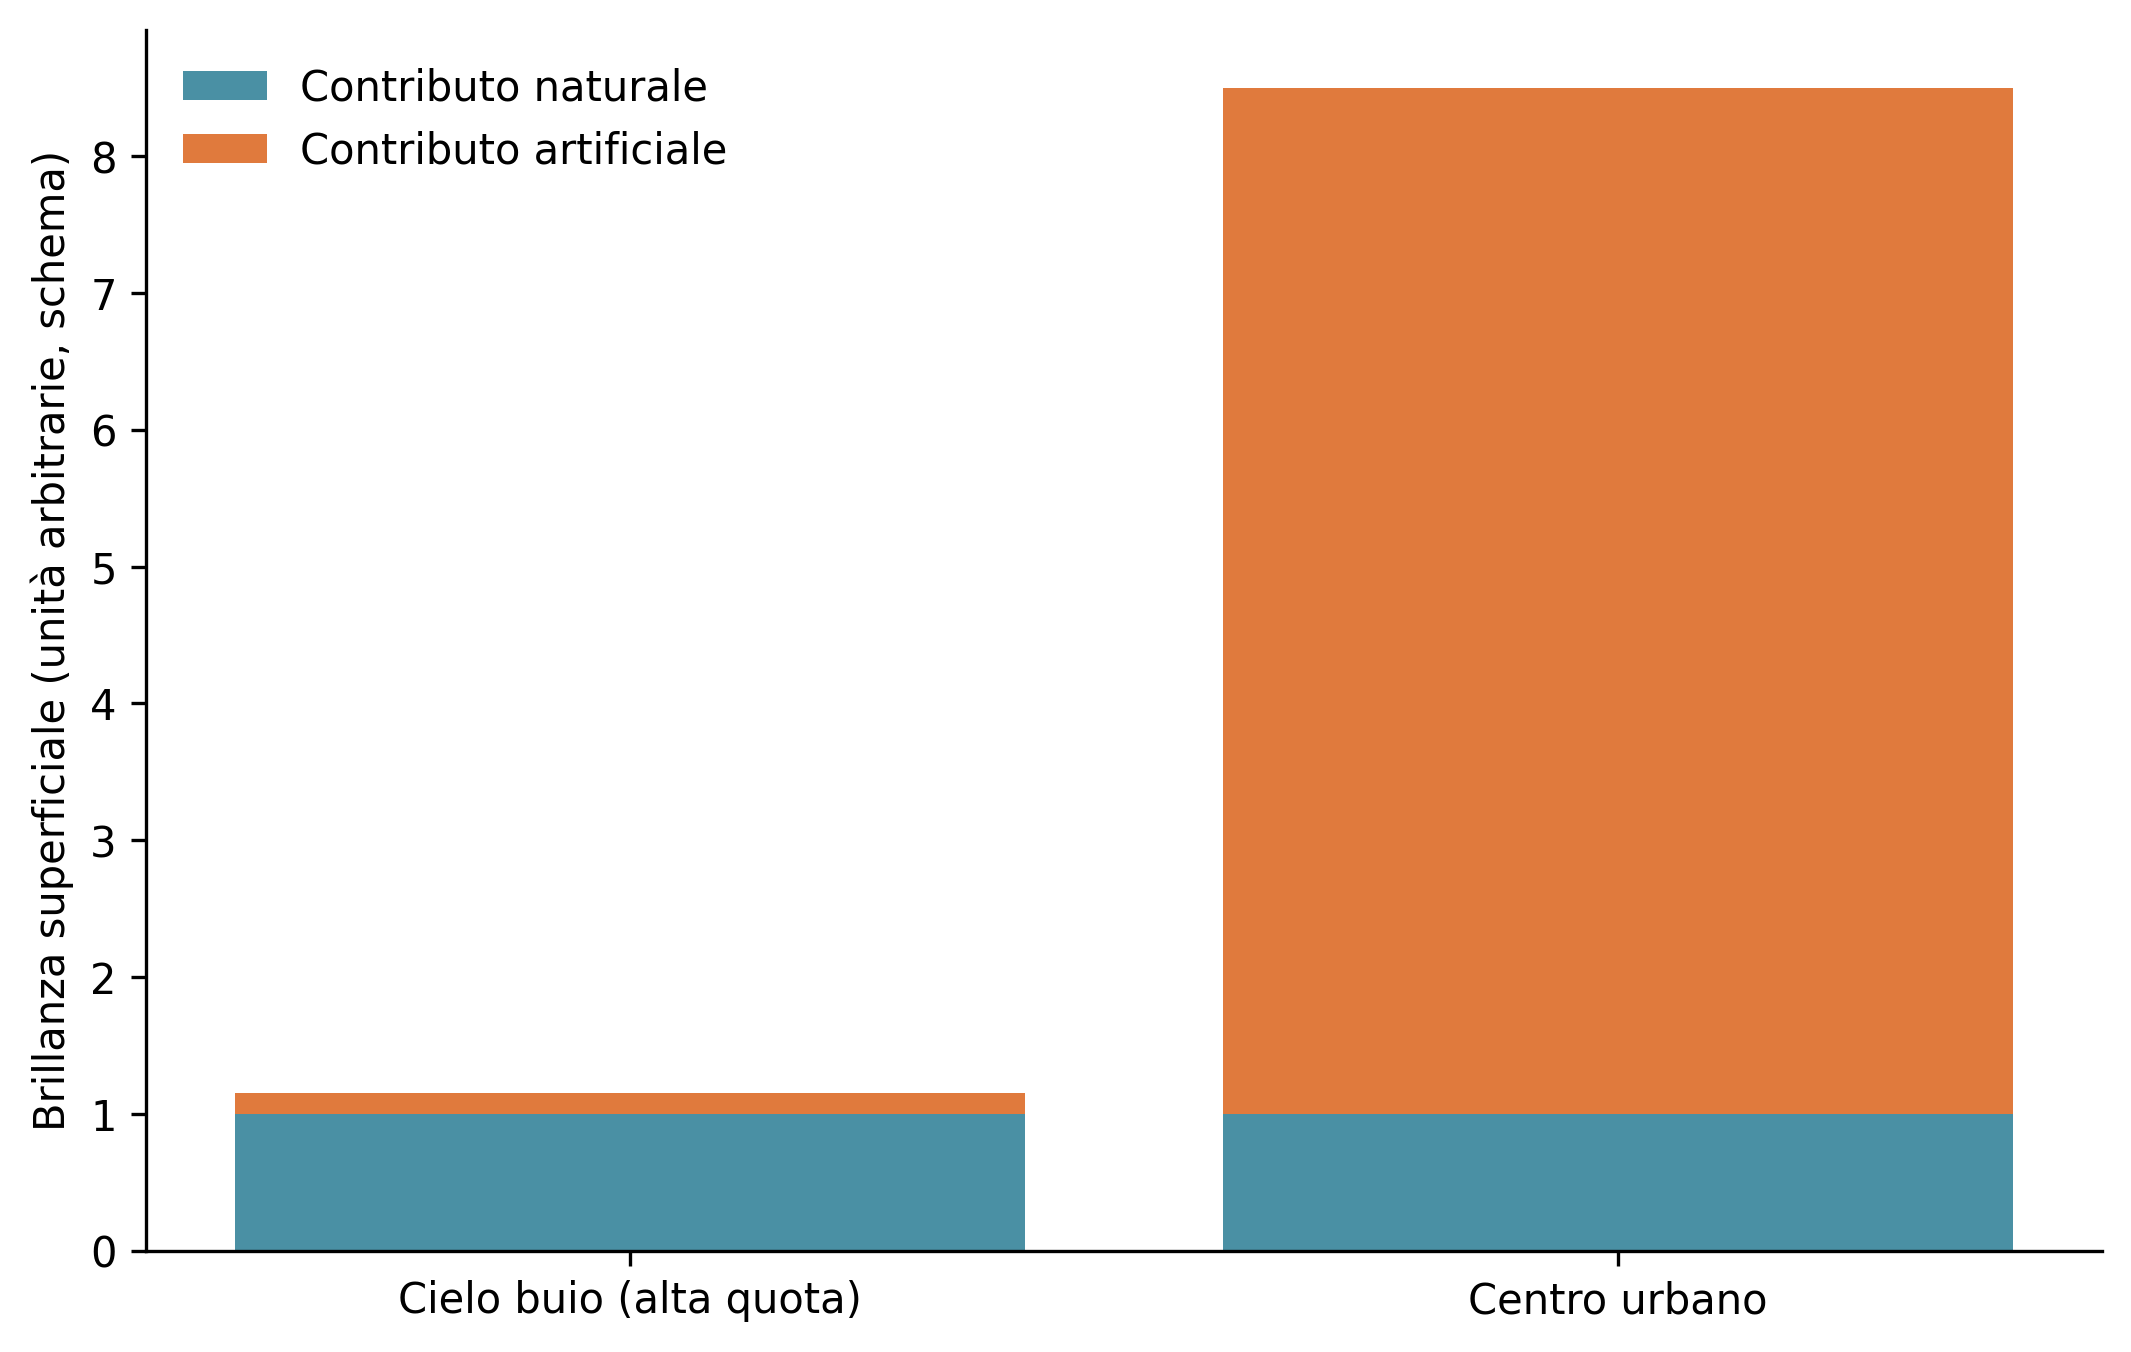
\includegraphics[width=0.92\textwidth]{figures/contributi_brillanza.png}
\caption{Schema della brillanza superficiale come somma di un contributo naturale e di un contributo artificiale. Le altezze delle barre sono illustrative, non misure di un sito specifico.}
\label{fig:contributi}
\end{figure}

Le mappe satellitari, in particolare lo strato \textit{VIIRS} (Visible Infrared Imaging Radiometer Suite), non misurano la brillanza del cielo zenitale. Quelle mappe riportano la radianza notturna uscente, cioè la luce che dalla superficie terrestre arriva al satellite, in nW\,cm$^{-2}$\,sr$^{-1}$. La radianza satellitare è un indicatore utile per collocare i nodi su un gradiente da città a montagna, e resta un osservabile diverso da quello del fotometro a terra. Nella comunicazione verso chi non lavora sul tema conviene mostrare una mappa a colori o un grafico, più immediati di una tabella di nanowatt.

\section*{Gli strumenti}
\addcontentsline{toc}{section}{Gli strumenti}

Per chi non lavora sul tema, una sigla come VIIRS o TESS-4C resta opaca. Conviene fissare 3 livelli di misura.

Dal satellite, il Day/Night Band di VIIRS fornisce composizioni annuali della radianza notturna, consultabili per esempio su \url{https://www.lightpollutionmap.info/}. La risoluzione è dell'ordine del chilometro; i pixel sotto 0,5\,nW\,cm$^{-2}$\,sr$^{-1}$ sono posti a 0 dal prodotto NASA. Lo strato satellitare serve a inquadrare il territorio, non a sostituire una misura locale.

A terra, i fotometri a zenit di basso costo (Sky Quality Meter, TESS-W e analoghi) puntano una porzione di cielo di circa 17$^{\circ}$ di campo e registrano una serie temporale di brillanza. Il TESS-W, sviluppato dal gruppo GUAIX dell'Universidad Complutense de Madrid nel progetto europeo STARS4ALL, è alloggiato in un contenitore stagno di 87$\times$75$\times$45\,mm, si alimenta via USB a 5\,V e trasmette i dati in WiFi con protocollo \texttt{MQTT}. La Figura~\ref{fig:tessw} mostra l'aspetto reale dello strumento, tratto dalla documentazione ufficiale. Lo strumento non è una cupola da osservatorio: l'ingombro è quello di un piccolo contenitore da esterno.

\begin{figure}[ht!]
\centering
% Immagine ufficiale STARS4ALL / GUAIX-UCM. Non generata dagli script di figura.
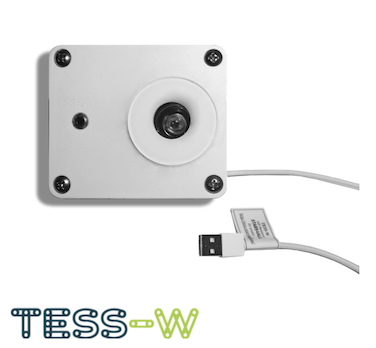
\includegraphics[width=0.55\textwidth]{figures/tess-w.png}
\caption{Fotometro TESS-W in contenitore stagno. Immagine ufficiale STARS4ALL / GUAIX-UCM.}
\label{fig:tessw}
\end{figure}

Un ulteriore livello è quello delle camere all-sky, che producono mappe di brillanza e di colore su tutta la volta. Restano strumenti da campagna o da osservatorio, non da rete capillare.

\section*{Il fotometro TESS-4C}
\addcontentsline{toc}{section}{Il fotometro TESS-4C}

Il TESS-4C è l'evoluzione a 4 bande del TESS-W: stesso ordine di grandezza dell'ingombro, stessa logica di installazione, 4 canali fotometrici caratterizzati al Laboratorio de Instrumentación Científica Avanzada (LICA-UCM). Il dato di colore consente di seguire, per esempio, la transizione dalle lampade al sodio ai LED. La Figura~\ref{fig:tess4c} riporta lo strumento e le curve di risposta dei 4 canali, dalla scheda tecnica GUAIX.

\begin{figure}[ht!]
\centering
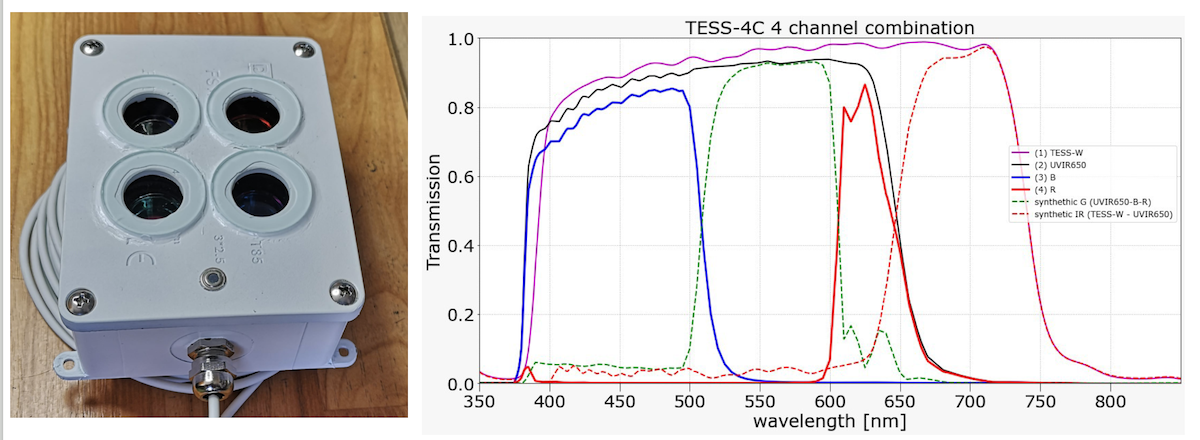
\includegraphics[width=\textwidth]{figures/tess-4c.png}
\caption{TESS-4C e curve di risposta dei 4 canali fotometrici. Fonte: GUAIX, Universidad Complutense de Madrid.}
\label{fig:tess4c}
\end{figure}

I dati sono resi disponibili in formato standard IDA-IAU e, in tempo reale, su pannelli Grafana della rete STARS4ALL. Per la rete abruzzese si aggiunge un cruscotto locale. I manuali della famiglia TESS (TESS-W, TESS-4C, TESS-P, TAS) sono disponibili in inglese, in spagnolo e in una traduzione italiana a supporto degli enti ospitanti.

Il costo indicativo del TESS-4C è di 550-650 EUR, IVA e spedizione comprese. L'ordine è effettuato direttamente dall'ente ospitante presso l'Universidad Complutense de Madrid.

\section*{Installazione}
\addcontentsline{toc}{section}{Installazione}

Chi non conosce la materia tende a immaginare una cupola sul tetto. Lo strumento è un contenitore di pochi centimetri, da fissare in esterno con vista libera dello zenit. L'installazione, tuttavia, non è banale: se arriva luce artificiale \textit{diretta} sul fotometro (un lampione, un'insegna, un faro di sicurezza), lo strumento misura quella sorgente, non la brillanza del cielo. La verifica va fatta in situ, di notte, prima del fissaggio definitivo.

La Figura~\ref{fig:installazione} confronta le 2 geometrie. A sinistra il fotometro è sul cornicione, esposto al lampione: un raggio diretto raggiunge l'ottica, il campo di vista verso lo zenit risulta contaminato e lo strumento registra la sorgente, non il cielo. A destra il fotometro è al centro del tetto, lontano dal bordo, con zenit libero; il lampione resta sotto il piano di falda e l'edificio lo scherma. L'alimentazione a 5\,V e la copertura WiFi restano necessarie, anche se non sono indicate nel disegno.

\begin{figure}[ht!]
\centering

\begin{tabular}{@{}cc@{}}
% Illustrazioni fisse di posa. Non generate dagli script di figura.
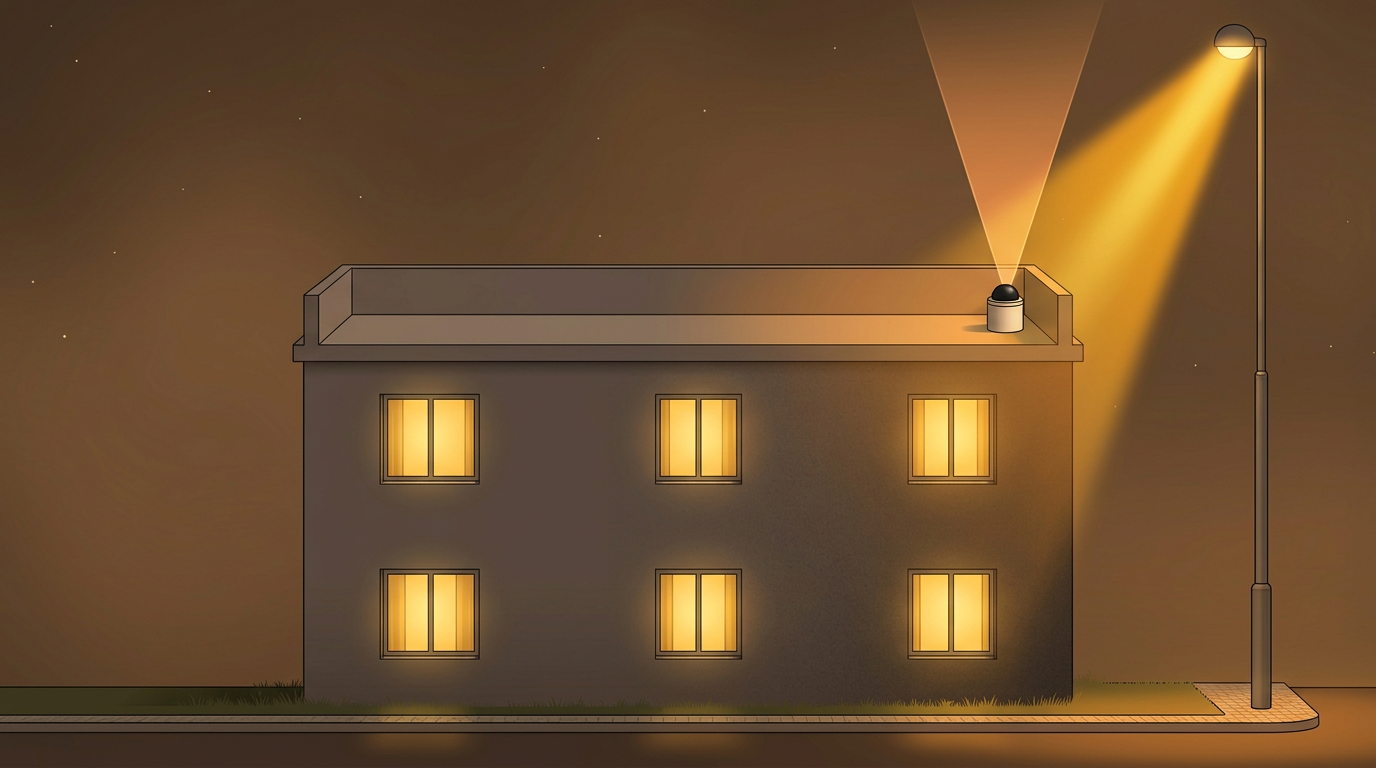
\includegraphics[width=0.48\textwidth]{figures/installazione_non_idonea.png} &
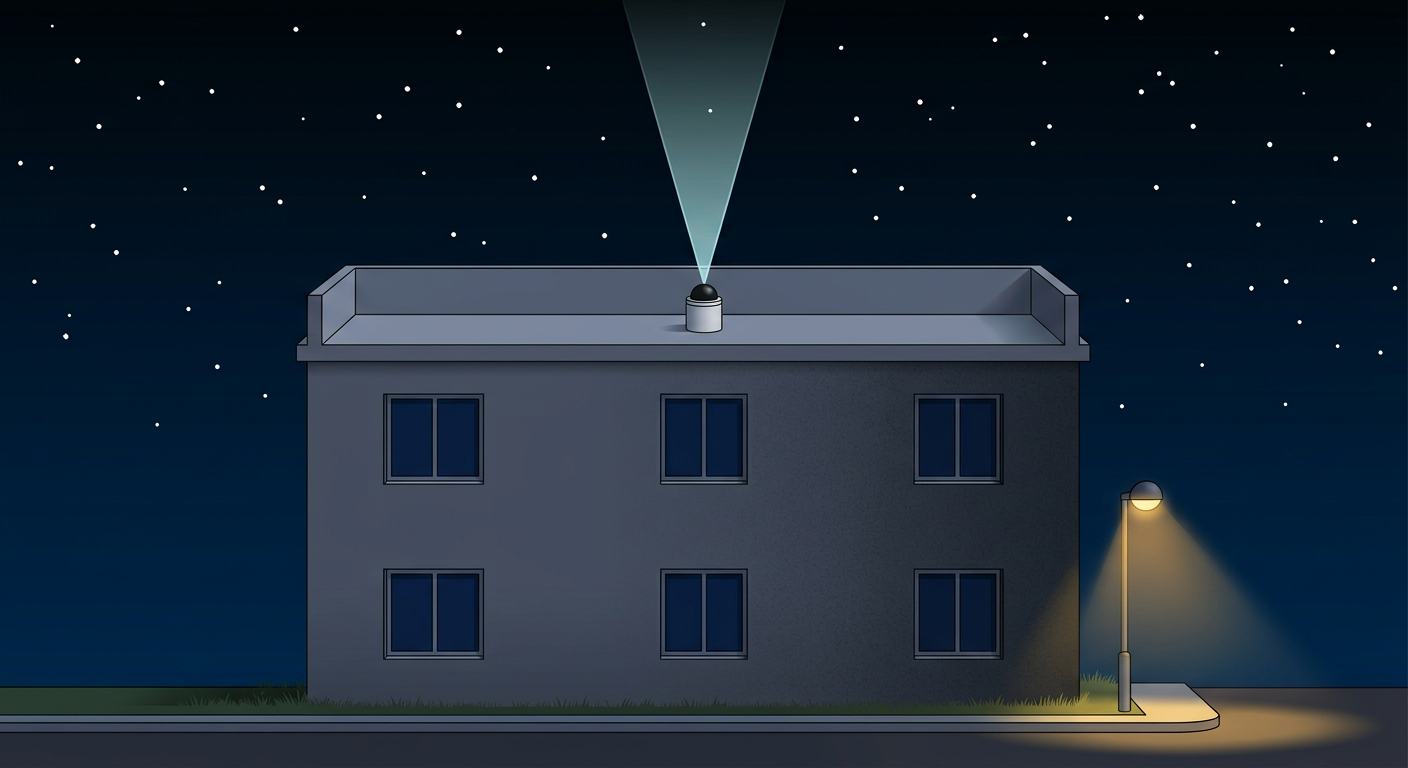
\includegraphics[width=0.48\textwidth]{figures/installazione_idonea.png}
\end{tabular}

\caption{Installazione del fotometro: geometria non idonea (sinistra) e geometria idonea (destra).}
\label{fig:installazione}
\end{figure}

L'installazione richiede 3 condizioni:

\begin{itemize}
\item alimentazione elettrica stabile, tipicamente 5\,V via USB, con consumo dell'ordine di 100 milliampere o più;
\item copertura WiFi verso un router che inoltri i dati (nei siti isolati si valuta un modulo dati alternativo);
\item assenza di luce artificiale diretta sul fotometro, proveniente da illuminazione pubblica o da qualsiasi altra sorgente.
\end{itemize}

Il referente di CieloBuio fornisce indicazioni e, se possibile, un sopralluogo. Il referente non esegue l'installazione: l'incarico resta a un tecnico scelto dall'ente ospitante.

\begin{table}[ht!]

\centering
\renewcommand{\arraystretch}{1.5}

\begin{tabularx}{\linewidth}{@{}l X@{}}
\toprule
Voce & Dettaglio \\
\midrule
Costo dello strumento & 550-650 EUR indicativi, IVA e spedizione comprese \\
Ingombro & contenitore stagno dell'ordine di 87$\times$75$\times$45\,mm (famiglia TESS) \\
Alimentazione & 5\,V USB \\
Connettività & WiFi, protocollo \texttt{MQTT}, repository STARS4ALL e cruscotto della rete abruzzese \\
Formato dati & serie IDA-IAU, pannelli Grafana in tempo reale \\
Sito & tetto, terrazza, rifugio o sede, con zenit libero e senza luce diretta \\
Manutenzione & verifica periodica di connettività e pulizia dell'ottica \\
\bottomrule
\end{tabularx}

\caption{Requisiti operativi comuni a tutti gli enti ospitanti.}
\label{tab:requisiti}
\end{table}

La Tabella~\ref{tab:requisiti} riassume i requisiti. Il protocollo di calibrazione periodica della rete viene definito per l'Abruzzo e comunicato a ciascun nodo.

% Seconda parte: solo da qui il testo si specializza sull'attore.
\section*{3 ambiti di collaborazione}
\addcontentsline{toc}{section}{3 ambiti di collaborazione}

Il preambolo precedente vale per tutti. Da qui il testo si specializza sull'attore. L'adesione resta volontaria e bilaterale: l'ente ospitante gestisce la propria stazione.

\subsection*{Istituti scolastici}

Per una scuola secondaria di primo o secondo grado la stazione è un laboratorio permanente. I dati servono in classe per statistica, grafici, confronto con altri nodi e andamento stagionale, in percorsi di fisica, scienze della terra, informatica ed educazione ambientale. La gestione della serie storica si presta a PCTO e a progetti di educazione civica, con un output pubblico: i dati confluiscono nella rete, non in un esercizio che si esaurisce a fine anno.

L'istituto resta autonomo nella scelta di come valorizzare didatticamente la stazione. L'istituto indica un docente referente e un punto di installazione sul tetto, in cortile o su una terrazza, verificato rispetto alla luce diretta.

\subsection*{Enti parco e aree protette}

Per un ente di tutela il cielo notturno è parte del patrimonio naturale, con effetti documentati su fauna notturna, migrazione, chirotteri e insetti impollinatori. Una serie continua di brillanza rende misurabile la qualità del buio e sostiene le politiche di gestione della luce artificiale, comprese eventuali zone di tutela rafforzata previste dalla disciplina regionale abruzzese.

Lo stesso dato è comunicabile a visitatori e strutture convenzionate. Se le condizioni di cielo lo consentono, le serie possono alimentare un futuro dossier per certificazioni internazionali, in particolare le riserve Starlight e i programmi Dark Sky. Nei rifugi in quota la connettività va valutata caso per caso.

\subsection*{Dipartimenti universitari}

Per un dipartimento di fisica (inclusa, ove presente, la fisica dell'atmosfera), di scienze ambientali o di astronomia, la stazione è una sorgente di dati fotometrici multibanda georeferenziati, utilizzabile per tesi, tirocini e pubblicazioni. Il confronto con i dati satellitari e la modellazione della propagazione della luce artificiale restano temi aperti.

Il dipartimento resta autonomo nella scelta dei temi di ricerca e nell'eventuale condivisione della paternità scientifica delle pubblicazioni. L'accesso ai dati grezzi è parte integrante della proposta.

\section*{I prossimi passi}
\addcontentsline{toc}{section}{I prossimi passi}

\begin{enumerate}
\item Un primo contatto, anche informale, per illustrare l'iniziativa e valutare il sito.
\item Individuazione condivisa del punto di installazione, con verifica di zenit libero, alimentazione, WiFi e assenza di luce diretta.
\item Acquisto dello strumento da parte dell'ente, sul canale ufficiale UCM.
\item Installazione a cura di un tecnico incaricato dall'ente, con supporto a distanza per la configurazione.
\item Attivazione nella rete abruzzese e comparsa dei dati sul cruscotto pubblico.
\end{enumerate}

\vspace{0.4cm}

\begin{center}
\begin{tikzpicture}
\draw[linegray, line width=0.6pt] (0,0) -- (12,0);
\end{tikzpicture}
\end{center}

\vspace{0.4cm}

\noindent\textit{Per informazioni e per fissare un primo contatto}:

\vspace{0.2cm}

\noindent Fabio Tempera, CieloBuio OdV

\url{fabiot2801@gmail.com} \quad $\cdot$ \quad 329 883 5142

\end{document}
